% =====================================================================
%  Cross-architecture generative scRNA-seq benchmark + biological-fidelity protocol
%  Application: NASA OSDR spaceflight transcriptomics (+ out-of-domain cancer control)
%  Target venue: npj Microgravity (Nature Portfolio)
%
%  SINGLE-FILE DRAFT. Compiles as-is with pdflatex (no external images or .bib needed).
%  - Figure slots are grey placeholder boxes; the real \includegraphics line is
%    commented directly beneath each so you can swap images in on Overleaf.
%  - Every number to be filled is wrapped in \res{...} and renders red for easy find/replace.
%  - Rename the protocol globally by editing \protname below.
% =====================================================================
\documentclass[11pt]{article}

\usepackage[utf8]{inputenc}
\usepackage[T1]{fontenc}
\usepackage[margin=1in]{geometry}
\usepackage{amsmath,amssymb}
\usepackage{graphicx}
\usepackage{xcolor}
\usepackage{booktabs}
\usepackage{array}
\usepackage{multirow}
\usepackage{caption}
\usepackage{authblk}
\usepackage{tikz}
\usetikzlibrary{positioning,arrows.meta,fit,backgrounds}
\usepackage[hidelinks]{hyperref}

% ---- Editable handles -------------------------------------------------
% Protocol name used throughout. Change once here to rename everywhere.
\newcommand{\protname}{biological-fidelity protocol}
\newcommand{\Protname}{Biological-fidelity protocol}
% Placeholder for any value you still need to fill (renders red).
\newcommand{\res}[1]{\textcolor{red}{[#1]}}
% Grey figure placeholder box.
\newcommand{\figplaceholder}[2]{%
  \fbox{\begin{minipage}[c][#1][c]{0.92\linewidth}\centering
  \color{gray}\itshape #2\end{minipage}}}
% -----------------------------------------------------------------------

\captionsetup{font=small,labelfont=bf}
\setlength{\parskip}{4pt}

\title{\bfseries Novel biological-fidelity metrics for evaluating synthetic single-cell RNA-seq, with the first application to spaceflight transcriptomics}

\author[1,2]{Arsh Suri\thanks{Corresponding author: suriarsh@gmail.com}}
\author[3]{Walter Alvarado}
\author[4]{James Casaletto}
\affil[1]{Wallace H.\ Coulter Department of Biomedical Engineering, Georgia Institute of Technology, Atlanta, GA, USA}
\affil[2]{Space Life Sciences Training Program, NASA Ames Research Center, Moffett Field, CA, USA}
\affil[3]{Space Biosciences Research Branch, NASA Ames Research Center, Moffett Field, CA, USA}
\affil[4]{Blue Marble Space Institute of Science, Seattle, WA, USA}

\date{}

\begin{document}
\maketitle

% =====================================================================
\begin{abstract}
\noindent
Spaceflight reshapes the transcriptome through microgravity, radiation, and circadian disruption, yet the cohorts available to study it are among the smallest in modern genomics, which limits statistical power and the development of predictive models for astronaut health. Deep generative models can augment these scarce datasets, but synthetic single-cell RNA sequencing (scRNA-seq) data has been judged almost entirely by distributional metrics that are blind to biology, and no peer-reviewed study has applied such models to spaceflight single-cell data. We introduce a \protname{} that scores three properties of synthetic data those metrics miss: overlap of the top differentially expressed genes between real and synthetic condition contrasts, overlap of enriched gene-ontology pathways computed with fgsea, and overlap of the most phenotypically predictive genes identified by random forests trained on synthetic versus real data under a train-on-synthetic, test-on-real design. To exercise the framework we generate synthetic data with three established architectures that span the main families of deep generative modeling, a conditional variational autoencoder (CVAE), the classifier-free latent diffusion model cfDiffusion, and a multi-conditional adaptation of scGAN, each conditioned on an identical covariate vector and each stopped at a common quality point defined by maximum mean discrepancy (MMD) convergence in a frozen principal-component space, so that the biological comparison reflects the generated data rather than unequal training. Applying the framework across \res{N} spaceflight configurations from the NASA Open Science Data Repository (OSDR), and to an out-of-domain cancer immune dataset as a robustness control, we find that the biological metrics separate models that distributional metrics rank as similar, that pathway-level fidelity exceeds gene-level fidelity, and that all models under-represent single-cell sparsity. This is, to our knowledge, the first application of generative augmentation and biology-aware evaluation to spaceflight single-cell transcriptomics, and the framework is dataset-agnostic and ready for adoption as spaceflight single-cell data grows.
\end{abstract}

% =====================================================================
\section{Introduction}

\subsection{Spaceflight remodels the transcriptome under uniquely constrained sampling}
Extended spaceflight alters human physiology through stressors absent from terrestrial evolution. Astronauts experience roughly 1.5\% monthly bone loss, cardiovascular deconditioning, and immune dysfunction, and these changes are accompanied by extensive transcriptomic reprogramming \cite{twins}. The NASA Twins Study found that over one thousand genes showed expression or epigenetic changes during flight, most of which returned toward baseline within six months, while a subset governing DNA repair, immune response, and bone formation remained altered \cite{twins}. The Inspiration4 mission and subsequent multi-omic atlases identified a recurring ``spaceflight signature'' spanning oxidative phosphorylation, immune function, and stress-response programs \cite{i4}. Single-cell resolution is increasingly central to resolving which cell populations drive these responses, but spaceflight single-cell datasets remain rare and small.

\subsection{Data scarcity is the binding constraint on spaceflight omics}
Fewer than six hundred people have flown in space, individual studies typically involve fewer than twenty subjects, and rodent missions are similarly limited once samples are stratified by tissue, sex, age, and mission \cite{ilangovan,scott}. The NASA Open Science Data Repository (OSDR) aggregates hundreds of transcriptomic datasets, yet small per-study sizes and preservation-related batch effects can eclipse the spaceflight signal itself \cite{osdr}. Prior NASA analyses have explicitly identified sample-power limitation as the central obstacle to applying machine learning in this domain, and have called for methods that cope with extreme sample scarcity \cite{scott,ilangovan}. Synthetic data augmentation is the standard remedy for exactly this regime.

\subsection{Generative models for scRNA-seq have proliferated but have not reached spaceflight, and are evaluated without biology}
Deep generative models for scRNA-seq now span variational autoencoders \cite{scvi,activa}, generative adversarial networks \cite{scgan}, and diffusion and flow-matching models \cite{scdiffusion,cfdiffusion,cfgen}, alongside analytical simulators \cite{scgft,scdesign3,simbench}. Two gaps persist. First, none of these methods has been applied, in a peer-reviewed study, to NASA OSDR spaceflight single-cell data; the only known artifact is an unpublished bulk RNA-seq GAN augmentation of GeneLab liver samples, which is neither single-cell nor a methods paper \cite{osdr}. Second, these models are compared almost exclusively through distributional similarity, for example maximum mean discrepancy, Fr\'echet-style distances, or a classifier two-sample test in which chance-level discrimination signals success \cite{scgan,scdiffusion}. Such metrics can be satisfied by data that is statistically plausible yet biologically hollow, preserving marginal distributions while losing the condition contrasts, mechanistic pathways, and predictive gene programs that make a dataset useful for discovery.

\subsection{Contributions}
This work makes two coupled contributions.

\noindent\textbf{A biological-fidelity evaluation framework.} We introduce a uniform, biology-aware evaluation of synthetic scRNA-seq built from three metrics that are absent from current practice: overlap of the top differentially expressed genes between real and synthetic condition contrasts (condition fidelity), overlap of enriched gene-ontology pathways from fgsea (mechanistic fidelity), and overlap of the most phenotypically predictive genes from random forests under a train-on-synthetic, test-on-real design (phenotypic fidelity). Together these ask whether synthetic data preserves the experimental contrast, the pathways that give the contrast its meaning, and the predictive gene programs, none of which is captured by the distributional metrics that dominate the field.

\noindent\textbf{The first application to spaceflight single-cell transcriptomics.} We apply generative augmentation and this evaluation to NASA OSDR spaceflight scRNA-seq, a domain where sample-power limitation is most severe and where, to our knowledge, no peer-reviewed generative single-cell study exists, directly addressing a limitation called out in prior NASA roadmaps \cite{scott,ilangovan}. To exercise the framework we use synthetic data from three established generators that span the main families, a CVAE, the classifier-free latent diffusion model cfDiffusion \cite{cfdiffusion}, and a multi-conditional adaptation of scGAN \cite{scgan}, each conditioned on an identical covariate vector and each stopped at a common quality point via MMD convergence so that the biological comparison is meaningful rather than an artifact of unequal training. Robustness is shown by applying the identical pipeline to an out-of-domain cancer immune dataset. These generators are existing, published methods used as a testbed; the contribution is the evaluation, not the models, and we neither propose a new generator nor claim to identify a best one. Where one architecture leads on biological fidelity we report it as a scoping observation, not a general ranking, since recent evidence on synthetic scRNA-seq is mixed \cite{cfgen,scgft,scdiffusion}.

% =====================================================================
\section{Results}

\subsection{A multi-model testbed for the protocol}
To exercise the \protname{} we generated synthetic data with three established generators that span the main families of deep generative modeling: a conditional variational autoencoder (CVAE), the classifier-free latent diffusion model cfDiffusion \cite{cfdiffusion}, and a multi-conditional adaptation of scGAN \cite{scgan}. These are existing, published methods; our purpose is to evaluate the synthetic data they produce, not to introduce or crown a generator. All three were trained on identical inputs, conditioned on an identical covariate vector, and stopped at a common quality point, so that any difference the biological metrics report reflects the fidelity of the generated data rather than unequal training (Fig.~\ref{fig:framework}; Methods). The evaluation is organized as a layered protocol: a statistical-fidelity layer based on MMD and complementary distances establishes that the generators reached comparable distributional quality, and three biological layers then ask, in turn, whether the synthetic data preserves the experimental contrast, the underlying pathways, and the predictive gene programs.

\begin{figure}[t]
\centering
\resizebox{\textwidth}{!}{%
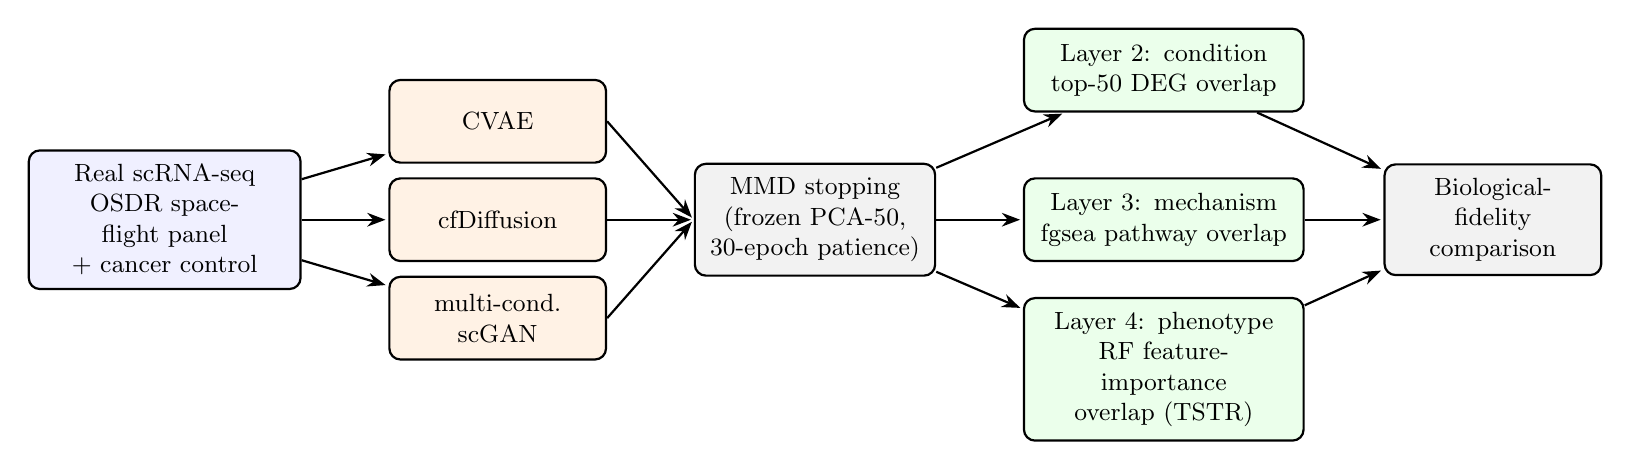
\begin{tikzpicture}[
  font=\small,
  box/.style={draw, rounded corners, align=center, inner sep=5pt, minimum height=1.05cm, text width=3.1cm},
  data/.style={box, fill=blue!6},
  model/.style={box, fill=orange!10, text width=2.4cm},
  stat/.style={box, fill=gray!10, text width=2.7cm},
  bio/.style={box, fill=green!8, text width=3.2cm},
  >={Stealth[]}, thick,
  arr/.style={->, shorten >=1pt}
]
% Data
\node[data] (data) {Real scRNA-seq\\OSDR spaceflight panel\\+ cancer control};
% Models
\node[model, right=1.1cm of data, yshift=1.25cm] (cvae) {CVAE};
\node[model, right=1.1cm of data] (diff) {cfDiffusion};
\node[model, right=1.1cm of data, yshift=-1.25cm] (gan) {multi-cond.\ scGAN};
% Stopping rule
\node[stat, right=1.1cm of diff] (mmd) {MMD stopping\\(frozen PCA-50,\\30-epoch patience)};
% Bio layers
\node[bio, right=1.1cm of mmd, yshift=1.9cm] (l2) {Layer 2: condition\\top-50 DEG overlap};
\node[bio, right=1.1cm of mmd, yshift=0.0cm] (l3) {Layer 3: mechanism\\fgsea pathway overlap};
\node[bio, right=1.1cm of mmd, yshift=-1.9cm] (l4) {Layer 4: phenotype\\RF feature-importance\\overlap (TSTR)};
% Score
\node[stat, right=1.0cm of l3, text width=2.4cm] (score) {Biological-\\fidelity\\comparison};

\draw[arr] (data) -- (cvae);
\draw[arr] (data) -- (diff);
\draw[arr] (data) -- (gan);
\draw[arr] (cvae.east) -- (mmd.west);
\draw[arr] (diff.east) -- (mmd.west);
\draw[arr] (gan.east) -- (mmd.west);
\draw[arr] (mmd) -- (l2);
\draw[arr] (mmd) -- (l3);
\draw[arr] (mmd) -- (l4);
\draw[arr] (l2) -- (score);
\draw[arr] (l3) -- (score);
\draw[arr] (l4) -- (score);
\end{tikzpicture}}
\caption{\textbf{The \protname{} and its multi-model testbed.} Synthetic data is generated by three representative generators trained on identical inputs with an identical conditioning vector and stopped at a common quality point by a shared MMD-convergence rule computed in a frozen 50-component PCA space (statistical-fidelity layer). Generated data then passes three biology-aware layers: condition preservation (top-50 differentially expressed gene overlap), mechanistic preservation (fgsea pathway overlap), and phenotypic preservation (random-forest feature-importance overlap under a train-on-synthetic, test-on-real design). The protocol is architecture-agnostic and dataset-agnostic.}
\label{fig:framework}
\end{figure}

\subsection{MMD convergence provides an architecture-agnostic stopping rule}
Loss values are not comparable across architectures: the CVAE optimizes an evidence lower bound, scGAN optimizes an adversarial Wasserstein objective whose magnitude is unbounded and does not track sample quality, and the diffusion model optimizes a denoising loss. Stopping each model on its own loss would compare the three at incommensurable operating points. We therefore stopped every model on the same external criterion, MMD between real and synthetic data measured in a frozen 50-component PCA space, halting when MMD failed to improve over a 30-epoch window (Fig.~\ref{fig:mmd}; Methods). Table~\ref{tab:stat} reports the MMD reached at convergence for each model and dataset, together with complementary distance metrics. Across datasets, \res{model} reached the lowest converged MMD, though the ranking on distance metrics was \res{consistent / mixed}, underscoring why a single distributional number is insufficient to declare a winner.

\begin{figure}[t]
\centering
\figplaceholder{5.2cm}{Figure placeholder: MMD convergence curves. \\ Per-architecture MMD (frozen PCA-50) versus training epoch for a representative dataset, with the 30-epoch no-improvement stopping point marked for each model.}
% 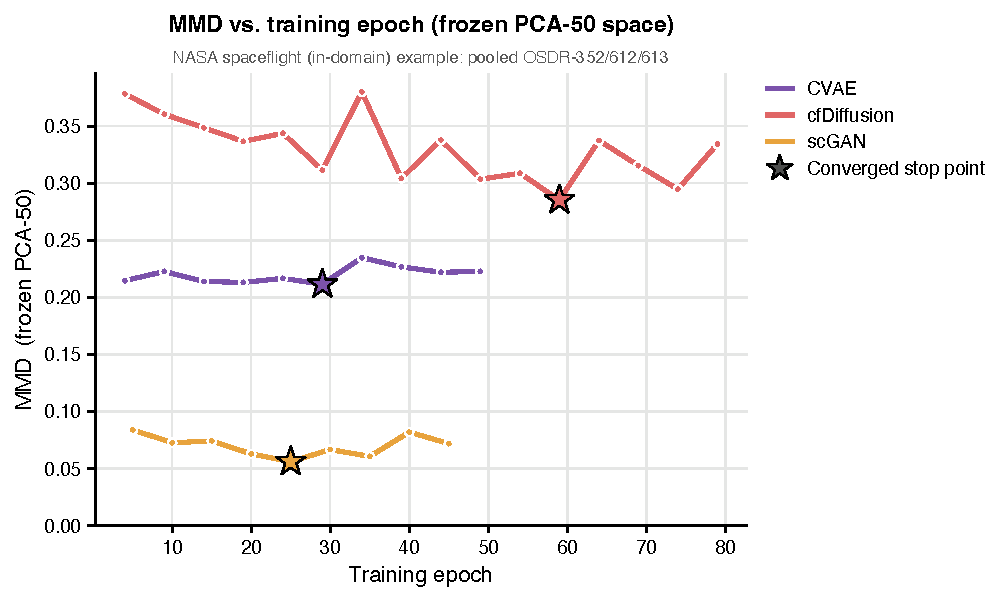
\includegraphics[width=0.9\linewidth]{fig_mmd_convergence.pdf}
\caption{\textbf{MMD-based stopping.} Maximum mean discrepancy between real and synthetic data, computed in a frozen 50-component PCA space, as a function of training epoch for the CVAE, cfDiffusion, and multi-conditional scGAN on a representative dataset. Training halts when MMD does not improve over 30 consecutive epochs (dashed markers). This yields an architecture-agnostic operating point at which the models are compared.}
\label{fig:mmd}
\end{figure}

\subsection{The models reconstruct global structure but not single-cell sparsity}
Low-dimensional embeddings show that synthetic cells overlap the real manifold to differing degrees across architectures (Fig.~\ref{fig:umap}). However, all three models generated data that was substantially less sparse than real single-cell data (Fig.~\ref{fig:sparsity}). Real datasets exhibited \res{approx.\ 92}\% zeros, consistent with technical dropout and biological stochasticity, whereas the diffusion model produced the densest output (\res{value}\% zeros), the CVAE was intermediate (\res{value}\% zeros), and scGAN reached \res{value}\% zeros. This over-densification is a shared limitation of latent-space generation and is examined in the Discussion, since it bears directly on which downstream analyses synthetic spaceflight data can currently support.

\begin{figure}[t]
\centering
\figplaceholder{5.6cm}{Figure placeholder: UMAP embeddings. \\ Real versus synthetic cells for representative spaceflight datasets, one panel per architecture, colored by condition (flight vs.\ ground) and by data source (real vs.\ synthetic).}
% \includegraphics[width=\linewidth]{fig_umap.pdf}
\caption{\textbf{Manifold overlap by architecture.} UMAP embeddings of real and synthetic cells for representative datasets. Columns correspond to the CVAE, cfDiffusion, and multi-conditional scGAN; points are colored by experimental condition and by real versus synthetic origin. \res{Describe the observed overlap and any architecture-specific separation once figures are inserted.}}
\label{fig:umap}
\end{figure}

\begin{figure}[t]
\centering
\figplaceholder{5.0cm}{Figure placeholder: sparsity comparison. \\ Distribution of per-cell (or per-gene) zero fraction for real data and for each generator, showing that synthetic data is systematically less sparse than real single-cell data.}
% 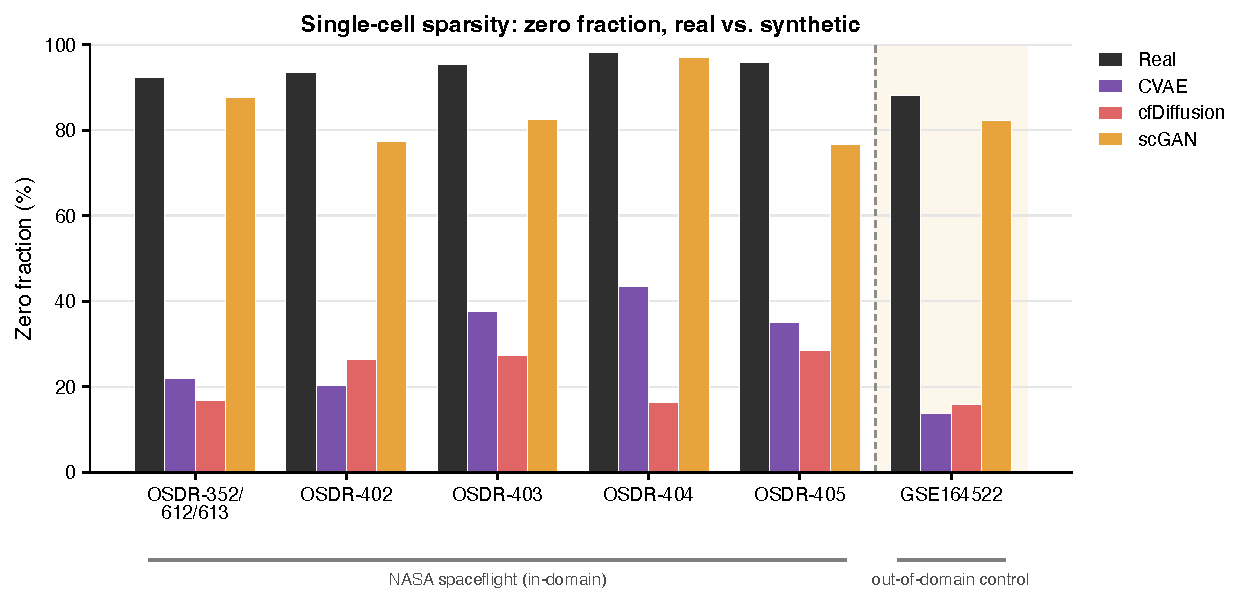
\includegraphics[width=0.85\linewidth]{fig_sparsity.pdf}
\caption{\textbf{Under-representation of single-cell sparsity.} Zero-fraction distributions for real data and for each generator. All architectures produce denser-than-real output; the diffusion model is densest, consistent with information loss in the latent bottleneck. Accurate dropout structure is required for cell-type identification and trajectory inference, which constrains the immediate use of the current synthetic data to bulk-like and pathway-level analyses.}
\label{fig:sparsity}
\end{figure}

\subsection{Condition fidelity: overlap of top differentially expressed genes}
For each dataset we identified the top 50 genes distinguishing flight from ground control, ranked by absolute log fold change, separately in real and synthetic data, and quantified their overlap (Methods). This asks whether the synthetic data preserves the biological contrast that motivates the experiment, a stronger test than overall distributional similarity. Overlap reached up to \res{approx.\ 50}\% for \res{scGAN}, exceeding the CVAE and cfDiffusion on \res{number}/\res{N} datasets (Table~\ref{tab:bio}; Fig.~\ref{fig:overlap}). The choice of $N=50$ is a convention rather than a constraint: the metric is defined for any top-$N$ list, and we report its sensitivity to $N$ in \res{Supplementary Fig.\ SX}.

\subsection{Mechanistic fidelity: fgsea pathway overlap}
Because two datasets can share biological function without sharing exact gene identities, we computed gene-ontology enrichment with fgsea on real and synthetic data and measured the overlap of significantly enriched pathways (Methods). Pathway overlap was consistently higher than gene-level overlap across architectures (Fig.~\ref{fig:fgsea}), indicating that the generators preserve coordinated transcriptional programs even where individual gene lists diverge. \res{scGAN / the diffusion model} recovered known spaceflight-associated programs, including \res{e.g., oxidative phosphorylation, translation and ribosomal pathways, stress response}, in \res{value}\% of cases. This layer is, to our knowledge, the first use of fgsea pathway overlap as a synthetic-data quality metric for generative-model comparison.

\subsection{Phenotypic fidelity: predictive-gene overlap under a train-on-synthetic design}
Finally we asked whether the synthetic data preserves the gene programs that are predictive of the phenotype. We trained random-forest classifiers to distinguish flight from ground control, one on synthetic data and one on real data, and compared their top-50 most important genes (Methods). This is a train-on-synthetic, test-on-real (TSTR) design, the opposite of the classifier two-sample test used in prior work: here high agreement, not chance-level discrimination, is the goal. Feature-importance overlap reached \res{value}\% for \res{model}, with \res{model} again leading (Table~\ref{tab:bio}). Absolute label-transfer performance was modest (TSTR AUC \res{value}, Table~\ref{tab:stat}), so we interpret this layer as evidence of preserved predictive gene structure rather than of turnkey classifier transfer. The overlap of important genes, rather than the raw AUC, is the informative quantity, because it reports whether the synthetic data encodes the same mechanistic basis for the prediction as the real data.

\subsection{The protocol is robust out of domain}
Applying the identical pipeline, with no retraining strategy, hyperparameter change, or metric modification, to the out-of-domain CANCER IMMU 10x dataset (\res{approx.\ 120{,}000+} cells, metastatic versus non-metastatic immune cells) produced \res{consistent / degraded} biological-fidelity behavior relative to the spaceflight datasets (Table~\ref{tab:bio}). This demonstrates that the \protname{} and the MMD-stopping rule are not tuned to spaceflight data and transfer to an unrelated single-cell domain, supporting their use as a general benchmark.

% ---------- Tables ----------
\begin{table}[t]
\centering
\caption{\textbf{Dataset panel.} Spaceflight configurations drawn from NASA OSDR, evaluated both as individual studies and as pooled cohorts, together with one out-of-domain cancer control. \res{Confirm accessions, tissues, cell counts, and the exact pooling scheme; the roster below reflects the current working set and should be verified before submission.}}
\label{tab:data}
\small
\resizebox{\textwidth}{!}{%
\begin{tabular}{@{}llccl@{}}
\toprule
Dataset (label) & Domain / tissue & Cells & Conditions & Notes \\
\midrule
Mouse brain (pooled) & Spaceflight, brain & \res{n} & \res{k} & Pooled OSD-612 / OSD-613 / OSD-352 \\
OSD-402 & Spaceflight, \res{tissue} & \res{n} & \res{k} & Individual study \\
OSD-403 & Spaceflight, \res{tissue} & \res{n} & \res{k} & Individual study \\
OSD-404 & Spaceflight, \res{tissue} & \res{n} & \res{k} & Individual study \\
OSD-405 & Spaceflight, \res{tissue} & \res{n} & \res{k} & Individual study \\
OSDR (pooled) & Spaceflight, multi-tissue & \res{n} & \res{k} & Pooled spaceflight cohort \\
CANCER IMMU 10x & Cancer, immune (10x) & \res{120{,}000+} & \res{k} & Out-of-domain control; metastatic vs.\ non-metastatic \\
\bottomrule
\end{tabular}}
\end{table}

\begin{table}[t]
\centering
\caption{\textbf{Statistical-fidelity layer.} MMD at convergence (frozen PCA-50) and complementary distance metrics per architecture and dataset, plus the secondary TSTR AUC. Lower is better for MMD, cosine distance, Wasserstein distance, MAD, and Mahalanobis distance. \res{Fill from your metrics table.}}
\label{tab:stat}
\small
\setlength{\tabcolsep}{5pt}
\resizebox{\textwidth}{!}{%
\begin{tabular}{@{}l l c c c c c c@{}}
\toprule
Dataset & Model & MMD$\downarrow$ & Cosine$\downarrow$ & Wasserstein$\downarrow$ & MAD$\downarrow$ & Mahal.$\downarrow$ & TSTR AUC \\
\midrule
\multirow{3}{*}{Mouse brain (pooled)}
 & CVAE        & \res{ } & \res{ } & \res{ } & \res{ } & \res{ } & \res{ } \\
 & cfDiffusion & \res{ } & \res{ } & \res{ } & \res{ } & \res{ } & \res{ } \\
 & scGAN       & \res{ } & \res{ } & \res{ } & \res{ } & \res{ } & \res{ } \\
\midrule
\multirow{3}{*}{OSD-402}
 & CVAE        & \res{ } & \res{ } & \res{ } & \res{ } & \res{ } & \res{ } \\
 & cfDiffusion & \res{ } & \res{ } & \res{ } & \res{ } & \res{ } & \res{ } \\
 & scGAN       & \res{ } & \res{ } & \res{ } & \res{ } & \res{ } & \res{ } \\
\midrule
\multicolumn{8}{c}{\itshape \res{$\ldots$ repeat rows for OSD-403, OSD-404, OSD-405, OSDR (pooled), CANCER IMMU 10x $\ldots$}} \\
\bottomrule
\end{tabular}}
\end{table}

\begin{table}[t]
\centering
\caption{\textbf{\Protname{} results.} Biological-fidelity metrics per dataset and architecture: top-50 DEG overlap (condition fidelity), fgsea pathway overlap (mechanistic fidelity), and random-forest feature-importance overlap (phenotypic fidelity, TSTR). Higher is better throughout; values are percentages. \res{Fill from your metrics table.}}
\label{tab:bio}
\small
\setlength{\tabcolsep}{5pt}
\resizebox{\textwidth}{!}{%
\begin{tabular}{@{}l ccc ccc ccc@{}}
\toprule
& \multicolumn{3}{c}{DEG overlap (\%)} & \multicolumn{3}{c}{fgsea overlap (\%)} & \multicolumn{3}{c}{Predictive-gene overlap (\%)} \\
\cmidrule(lr){2-4}\cmidrule(lr){5-7}\cmidrule(lr){8-10}
Dataset & CVAE & cfDiff & scGAN & CVAE & cfDiff & scGAN & CVAE & cfDiff & scGAN \\
\midrule
Mouse brain (pooled) & \res{} & \res{} & \res{} & \res{} & \res{} & \res{} & \res{} & \res{} & \res{} \\
OSD-402              & \res{} & \res{} & \res{} & \res{} & \res{} & \res{} & \res{} & \res{} & \res{} \\
OSD-403              & \res{} & \res{} & \res{} & \res{} & \res{} & \res{} & \res{} & \res{} & \res{} \\
OSD-404              & \res{} & \res{} & \res{} & \res{} & \res{} & \res{} & \res{} & \res{} & \res{} \\
OSD-405              & \res{} & \res{} & \res{} & \res{} & \res{} & \res{} & \res{} & \res{} & \res{} \\
OSDR (pooled)        & \res{} & \res{} & \res{} & \res{} & \res{} & \res{} & \res{} & \res{} & \res{} \\
CANCER IMMU 10x      & \res{} & \res{} & \res{} & \res{} & \res{} & \res{} & \res{} & \res{} & \res{} \\
\bottomrule
\end{tabular}}
\end{table}

\begin{figure}[t]
\centering
\figplaceholder{5.0cm}{Figure placeholder: gene-overlap summary. \\ Grouped bars of top-50 DEG overlap and random-forest predictive-gene overlap across datasets (x-axis) and architectures (color).}
% 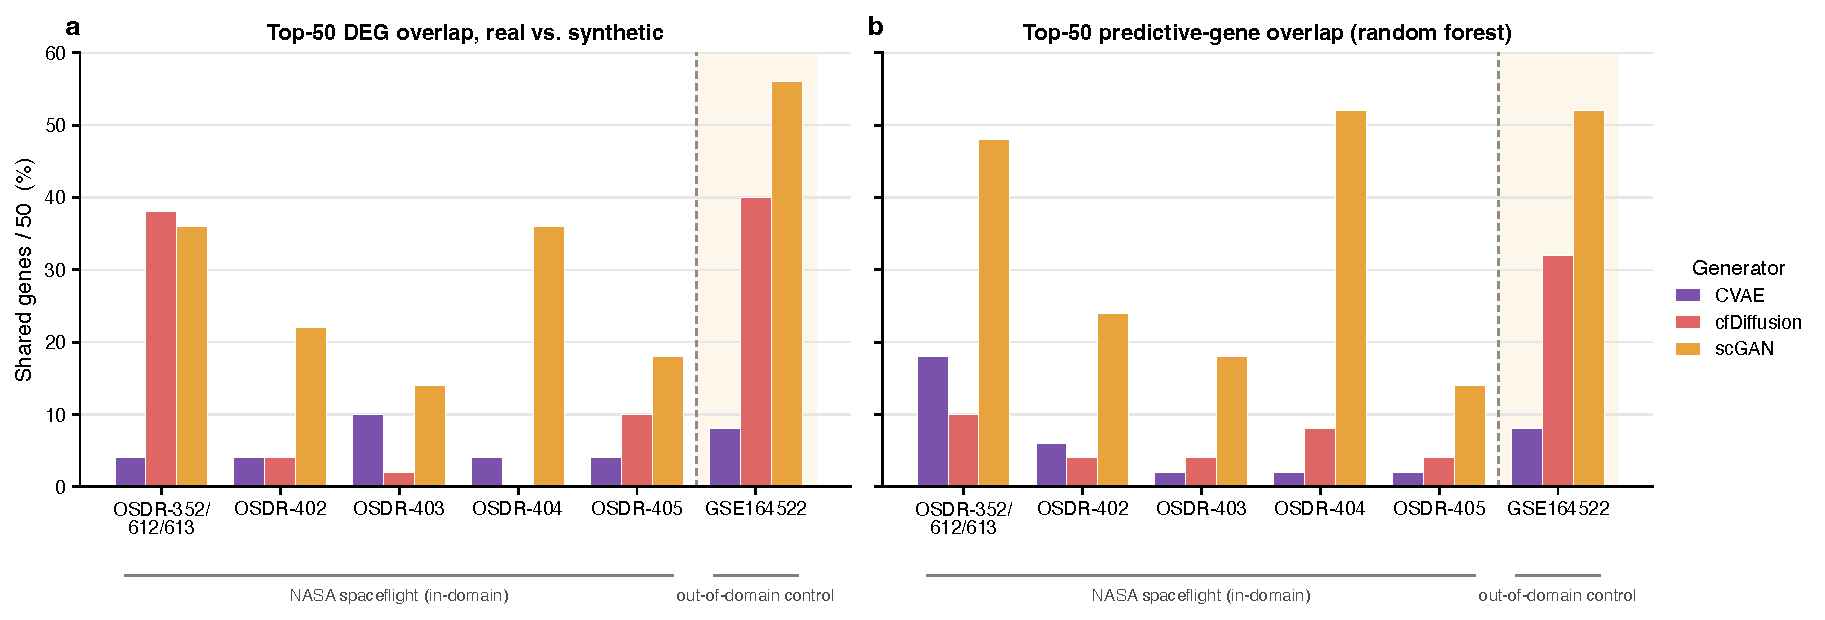
\includegraphics[width=\linewidth]{fig_overlap.pdf}
\caption{\textbf{Condition and phenotype fidelity across datasets.} Top-50 differentially expressed gene overlap and random-forest feature-importance overlap between real and synthetic data, grouped by dataset and architecture. \res{Summarize the leading architecture and the spread across datasets once inserted.}}
\label{fig:overlap}
\end{figure}

\begin{figure}[t]
\centering
\figplaceholder{5.0cm}{Figure placeholder: fgsea pathway overlap. \\ Real versus synthetic enriched-pathway overlap (e.g.\ heatmap or bar chart) for one representative dataset, or across all datasets and architectures.}
% 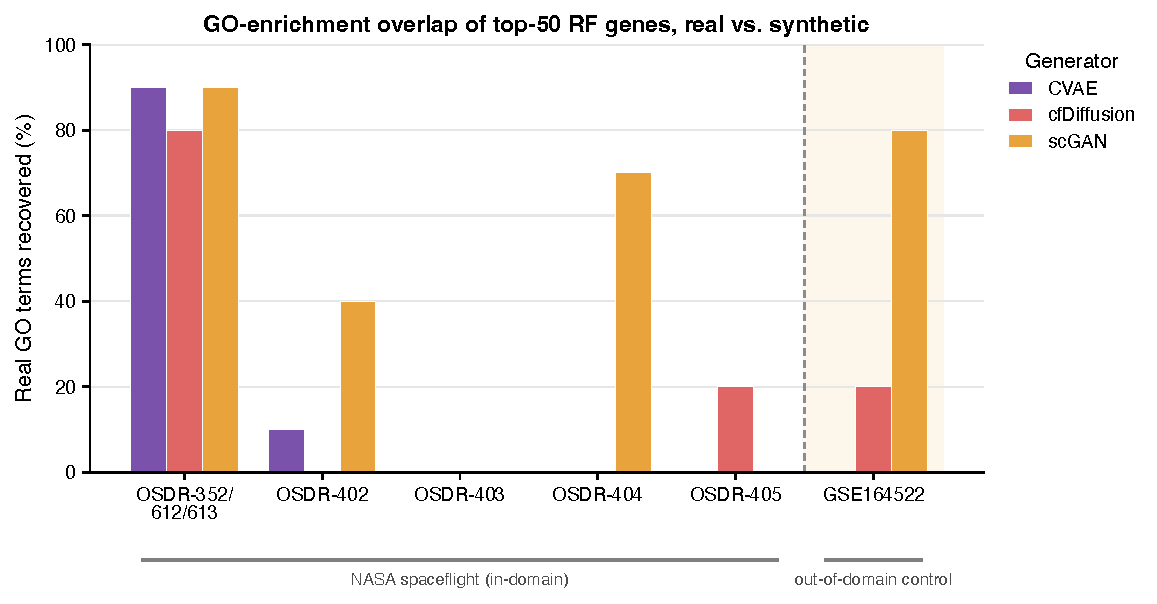
\includegraphics[width=\linewidth]{fig_fgsea.pdf}
\caption{\textbf{Mechanistic fidelity via fgsea.} Overlap of significantly enriched gene-ontology pathways between real and synthetic data. Pathway overlap exceeds gene-level overlap across architectures, indicating preservation of coordinated transcriptional programs. \res{Name the recovered spaceflight-associated pathways once inserted.}}
\label{fig:fgsea}
\end{figure}

% =====================================================================
\section{Discussion}

\subsection{Biological metrics separate what distributional metrics cannot}
Under a purely distributional lens the generators are difficult to tell apart, and they reached similar MMD at convergence. The \protname{} separates them by asking whether the synthetic data preserves the experimental contrast, the underlying pathways, and the predictive gene programs. This is the central point of the work: statistical similarity is necessary but not sufficient, and an evaluation that stops at distributional metrics can certify synthetic data that has quietly lost the biology it was meant to reproduce. Where architectures differed on these axes the multi-conditional scGAN tended to lead, which we report as a scoping observation on small-sample, multi-conditional data rather than a general ranking, since recent evidence on synthetic scRNA-seq is genuinely mixed \cite{scdiffusion,cfgen,scgft}.

\subsection{Why each layer is necessary}
The layers are ordered to catch distinct failure modes. A model can match the marginal distribution yet scramble the flight-versus-ground contrast; it can preserve the contrast yet miss the pathways that give the contrast meaning; and it can pass all of these yet fail to encode the gene programs that make the data predictive. Gene-level overlap and pathway-level overlap diverged in our data, with pathway overlap higher, which is precisely the mechanistic-but-not-mechanical fidelity that matters for discovery. A benchmark that reports only one of these numbers would misrepresent the usefulness of the synthetic data.

\subsection{The sparsity gap constrains current use}
All three models under-represented dropout, with the diffusion model densest. This over-densification follows from generating in a compressed latent space that discards fine-grained zero structure. The practical consequence is that the present synthetic data is suited to bulk-like and pathway-level analyses rather than to tasks that depend on accurate dropout, such as cell-type identification and trajectory inference. Sparsity-aware objectives, dropout-preserving latent variables analogous to library-size modeling in scVI \cite{scvi}, or count-based likelihoods are natural next steps.

\subsection{Limitations}
Several limitations bound our claims. The ``first peer-reviewed'' framing is contingent on the unpublished NASA bulk RNA-seq GAN artifact not appearing as a methods paper before submission, and we cite it transparently \cite{osdr}. The dataset panel, while at or above the size used by comparable methods papers \cite{cfgen,scdiffusion,cfdiffusion}, remains modest, and we therefore report the spread of metrics across datasets rather than single point estimates. The absolute TSTR AUC is limited, so we lead with feature-importance overlap rather than label-transfer performance. Finally, fgsea pathway overlap is a new synthetic-data metric and would benefit from further validation against held-out biological signal recovery. We view establishing this methodological foundation as timely, given that larger spaceflight single-cell datasets are only now becoming available.

\subsection{Implications for spaceflight medicine}
Condition-controllable synthetic cells enable in silico cohorts that are impossible to collect from astronauts, supporting power analyses, countermeasure screening across genetic backgrounds, and the development of predictive health models under the sample scarcity that defines this field \cite{scott,ilangovan}. The \protname{} gives the community a way to decide which synthetic data is trustworthy enough for these purposes, and the MMD-stopping rule gives a fair basis for choosing among generators as new architectures arrive.

% =====================================================================
\section{Methods}

\subsection{Datasets and preprocessing}
Spaceflight scRNA-seq datasets were obtained from NASA OSDR and evaluated both as individual studies and as pooled cohorts, alongside one out-of-domain cancer immune dataset (CANCER IMMU 10x) used as a robustness control (Table~\ref{tab:data}). The pooled mouse-brain configuration combines OSD-612, OSD-613, and OSD-352. \res{Specify the remaining accessions, tissues, subject counts, and the exact pooling scheme.} Count matrices were generated with Cell Ranger and filtered with standard per-cell quality thresholds \cite{tenx}. Counts were library-size normalized to $10^4$ and log$(x+1)$ transformed. Lowly expressed genes were removed (\res{state the threshold, e.g.\ genes detected in fewer than a set fraction of cells; a $0.997$ / $3\sigma$ cutoff was used}), and the top 2000 highly variable genes were selected with the Seurat variance-stabilizing transform \cite{seurat}. Each dataset was split into 80\% training, 10\% validation, and 10\% held-out test, stratified by experimental condition; biological-fidelity metrics were computed on the held-out test data to avoid optimistic assessment.

\subsection{Shared conditioning vector}
All three generators conditioned on an identical covariate vector, so that the biological comparison reflects the generated data and not differences in conditioning power: experimental condition (flight versus ground control), biological strain, sex, age at launch, and mission duration. Categorical variables were encoded as learned or one-hot embeddings and continuous variables were normalized, and the same encoded vector was supplied to every model. This symmetry removes conditioning power as a confounder across the testbed.

\subsection{Conditional variational autoencoder}
The CVAE maps 2000-gene expression vectors to a 50-dimensional latent space through fully connected layers with batch normalization and nonlinear activations, with the conditioning vector concatenated to the input and again to the latent code before decoding. It maximizes the conditional evidence lower bound,
\begin{equation}
\mathcal{L}_{\mathrm{CVAE}} = \mathbb{E}_{q_\phi(z\mid x,c)}\left[\log p_\theta(x\mid z,c)\right] - \beta\, D_{\mathrm{KL}}\!\left(q_\phi(z\mid x,c)\,\|\,p(z)\right),
\end{equation}
with a Gaussian posterior $q_\phi(z\mid x,c)=\mathcal{N}(z;\mu_\phi(x,c),\sigma_\phi^2(x,c))$, the reparameterization trick for differentiable sampling, a reconstruction term appropriate for normalized expression, and $\beta=\res{0.05}$ controlling the Kullback-Leibler regularization. Implemented in PyTorch.

\subsection{Classifier-free latent diffusion (cfDiffusion)}
Following cfDiffusion \cite{cfdiffusion}, a first-stage variational autoencoder compresses the 2000-gene vectors to a 128-dimensional latent space (encoder $1024\to1024\to128$, decoder reversed), and a second-stage denoising diffusion model operates in that latent space using a skip-connected network. The forward process adds Gaussian noise over $T=1000$ steps with schedule $\{\beta_t\}$, $q(z_t\mid z_{t-1})=\mathcal{N}(z_t;\sqrt{1-\beta_t}\,z_{t-1},\beta_t I)$, and the network $\epsilon_\theta(z_t,t,c)$ learns to predict the added noise by minimizing
\begin{equation}
\mathcal{L}_{\mathrm{diff}} = \mathbb{E}_{z_0,c,t,\epsilon}\left[\left\|\epsilon - \epsilon_\theta\!\left(\sqrt{\bar\alpha_t}\,z_0 + \sqrt{1-\bar\alpha_t}\,\epsilon,\; t,\; c\right)\right\|^2\right].
\end{equation}
Classifier-free guidance is enabled by dropping the condition with probability $p_{\mathrm{drop}}=0.15$ during training and combining conditional and unconditional predictions at inference, $\tilde\epsilon_\theta = \epsilon_\theta(z_t,t,\varnothing) + \gamma\left(\epsilon_\theta(z_t,t,c)-\epsilon_\theta(z_t,t,\varnothing)\right)$. Rectified activations are applied at inference only, so that negative gradients can flow during training while final generated expression remains non-negative. Categorical and continuous conditions are handled by separate embedding networks combined by projection and additive integration. Implemented in PyTorch.

\subsection{Multi-conditional scGAN}
The GAN arm is the scGAN architecture of Marouf et al.\ \cite{scgan}, a Wasserstein GAN with gradient penalty and a library-size normalization layer, implemented in TensorFlow. The original conditional variant (cscGAN) conditions on a single categorical variable (cell type). We extended it to accept the full multi-attribute conditioning vector used by the other two generators, injecting the covariates via \res{projection-based conditioning / conditional batch normalization / concatenated embeddings; confirm the exact mechanism} so that generation is controllable on condition, strain, sex, age, and duration jointly. This adaptation simply lets scGAN accept the same conditioning vector as the CVAE and cfDiffusion, which is what the evaluation requires; it is a means to a fair comparison rather than a modeling contribution in itself.

\subsection{MMD-based, architecture-agnostic stopping rule}
Because ELBO, adversarial, and denoising losses are not comparable across families, we stopped all models on a shared external criterion. We fit a 50-component principal-component analysis once on the real training data only and froze it. The same frozen transform was applied to both real validation data and synthetic data; MMD was never computed in the raw high-dimensional space, where distance concentration renders the radial-basis-function kernel insensitive, nor was the PCA ever refit on synthetic or pooled data. At fixed epoch intervals during training, the model generated a synthetic replicate of the validation set, both real and synthetic validation sets were projected through the frozen PCA, and MMD was computed between them with an RBF kernel \cite{gretton,sutherland}. The kernel bandwidth $\sigma$ was set by the median heuristic on the training data using proportional stratified sampling. Training continued while MMD improved and stopped when it failed to improve over a 30-epoch window, giving each generator its own converged operating point. This use of MMD as a shared stopping criterion, so that generators of different families reach a common quality point rather than being halted on incommensurable losses, is a deliberate choice that makes the biological comparison fair: MMD has been used as an evaluation metric \cite{gretton,sutherland} and as a within-family early-stopping signal, but here it serves as the common operating point at which otherwise incomparable generators are evaluated.

\subsection{Biological-fidelity protocol}
For every dataset and architecture we generated a full one-to-one replicate of the real dataset, matching the exact distribution of mission parameters (the same combinations of condition, strain, sex, age, and duration), and computed three metrics on held-out test data.

\noindent\textbf{Condition fidelity (DEG overlap).} Differential expression between flight and ground control was computed by t-test separately in real and synthetic data, genes were ranked by absolute log fold change, and the overlap of the top 50 genes was quantified. The value $N=50$ is a convention; the metric is defined for any $N$, and its sensitivity to $N$ is reported in \res{Supplementary Fig.\ SX}.

\noindent\textbf{Mechanistic fidelity (fgsea overlap).} Preranked gene-set enrichment analysis was performed with fgsea \cite{fgsea} against gene-ontology gene sets, separately for real and synthetic data, and the overlap of significantly enriched pathways was measured. This captures functional coherence that gene-level overlap can miss.

\noindent\textbf{Phenotypic fidelity (RF feature-importance overlap, TSTR).} Random-forest classifiers were trained to distinguish flight from ground control, one on synthetic data and one on real data, and their top 50 most important genes were compared by overlap. Training on synthetic data and testing on real held-out data (train-on-synthetic, test-on-real \cite{esteban}) inverts the classifier two-sample test of prior work \cite{scgan,scdiffusion,lopezpaz}, in which chance-level discrimination is optimal: here, high agreement is optimal. Because absolute TSTR AUC was modest, we report feature-importance overlap as the primary phenotypic-fidelity quantity and AUC as a secondary measure.

\subsection{Statistical-fidelity distances}
Alongside MMD we report cosine distance, Wasserstein distance (Sinkhorn-approximated), mean absolute deviation of per-gene means, and Mahalanobis distance using the pooled covariance, providing complementary views of local and global distributional similarity.

\subsection{Training and hardware}
Models used Adam optimization (learning rate $10^{-3}$ for the CVAE and $2\times10^{-4}$ for diffusion; \res{learning rate} for scGAN) with the MMD stopping rule above. \res{State batch sizes, guidance strength $\gamma$, gradient-penalty weight, and total epochs to convergence per model.} Experiments used NVIDIA A100 GPUs. For evaluation, each model generated a one-to-one synthetic replicate of the corresponding real dataset; diffusion sampling used DDIM with \res{number} steps.

\subsection{Code and data availability}
All scRNA-seq datasets are available in the NASA OSDR \cite{osdr}. Training scripts, trained models, generated data, and the \protname{} implementation are available at \res{repository URL}.

% =====================================================================
\section*{Acknowledgements}
We thank the Space Life Sciences Training Program and the AI4LS team at NASA Ames Research Center for support. \res{Add grant numbers, VIP program acknowledgement, and any additional personnel.}

\section*{Author contributions}
\res{Specify, e.g.: A.S.\ conceived the study, implemented the models and the biological-fidelity protocol, ran experiments, and wrote the manuscript; W.A.\ and J.C.\ supervised and edited.}

\section*{Competing interests}
The authors declare no competing interests.

% =====================================================================
\begin{thebibliography}{99}
\small
\bibitem{twins} Garrett-Bakelman FE, et al. The NASA Twins Study: a multidimensional analysis of a year-long human spaceflight. \textit{Science} 364, eaau8650 (2019). doi:10.1126/science.aau8650.
\bibitem{i4} Overbey EG, et al. Spatial and single-cell profiling of the multiomic response to spaceflight. \textit{Nat.\ Commun.} 15, 4954 (2024). doi:10.1038/s41467-024-48916-8.
\bibitem{ilangovan} Ilangovan V, et al. Machine learning classification of spaceflown versus ground-control mice from harmonized liver transcriptomes. \textit{npj Microgravity} 10, 61 (2024). doi:10.1038/s41526-024-00379-3.
\bibitem{scott} Scott RT, Sanders LM, Antonsen EL, et al. Biomonitoring and precision health in deep space supported by artificial intelligence. \textit{Nat.\ Mach.\ Intell.} 5, 196--207 (2023). doi:10.1038/s42256-023-00618-4.
\bibitem{osdr} Gebre SG, et al. NASA Open Science Data Repository: open science for life in space. \textit{Nucleic Acids Res.} 53, D1697--D1710 (2024). doi:10.1093/nar/gkae1116.
\bibitem{scvi} Lopez R, Regier J, Cole MB, Jordan MI, Yosef N. Deep generative modeling for single-cell transcriptomics. \textit{Nat.\ Methods} 15, 1053--1058 (2018). doi:10.1038/s41592-018-0229-2.
\bibitem{activa} Heydari AA, Davalos OA, Zhao L, Hoyer KK, Sindi SS. ACTIVA: realistic single-cell RNA-seq generation with automatic cell-type identification using introspective variational autoencoders. \textit{Bioinformatics} 38, 2194--2201 (2022). doi:10.1093/bioinformatics/btac095.
\bibitem{scgan} Marouf M, et al. Realistic in silico generation and augmentation of single-cell RNA-seq data using generative adversarial networks. \textit{Nat.\ Commun.} 11, 166 (2020). doi:10.1038/s41467-019-14018-z.
\bibitem{scdiffusion} Luo E, Hao M, Wei L, Zhang X. scDiffusion: conditional generation of high-quality single-cell data using diffusion model. \textit{Bioinformatics} 40, btae518 (2024). doi:10.1093/bioinformatics/btae518.
\bibitem{cfdiffusion} Zhang T, Zhao Z, Ren J, Zhang Z, Zhang H, Wang G. cfDiffusion: diffusion-based efficient generation of high-quality scRNA-seq data with classifier-free guidance. \textit{Brief.\ Bioinform.} 26, bbaf071 (2025). doi:10.1093/bib/bbaf071.
\bibitem{cfgen} Palma A, et al. Multi-modal and multi-attribute generation of single cells with CFGen. \textit{Proc.\ ICLR} (2025). arXiv:2407.11734.
\bibitem{scgft} Tedesco M, et al. Single-cell generative modeling with the Fourier transform (scGFT). \textit{Commun.\ Biol.} 8, 1 (2025). doi:10.1038/s42003-025-07552-8.
\bibitem{scdesign3} Song D, et al. scDesign3 generates realistic in silico data for multimodal single-cell and spatial omics. \textit{Nat.\ Biotechnol.} 41, 1610--1618 (2023). doi:10.1038/s41587-023-01772-1.
\bibitem{simbench} Cao Y, Yang P, Yang JYH. A benchmark study of simulation methods for single-cell RNA sequencing data. \textit{Nat.\ Commun.} 12, 6911 (2021). doi:10.1038/s41467-021-27130-w.
\bibitem{gretton} Gretton A, Borgwardt KM, Rasch MJ, Sch\"olkopf B, Smola A. A kernel two-sample test. \textit{J.\ Mach.\ Learn.\ Res.} 13, 723--773 (2012).
\bibitem{sutherland} Sutherland DJ, et al. Generative models and model criticism via optimized maximum mean discrepancy. \textit{Proc.\ ICLR} (2017). arXiv:1611.04488.
\bibitem{fgsea} Korotkevich G, Sukhov V, Sergushichev A. Fast gene set enrichment analysis. \textit{bioRxiv} 060012 (2021). doi:10.1101/060012.
\bibitem{esteban} Esteban C, Hyland SL, R\"atsch G. Real-valued (medical) time series generation with recurrent conditional GANs. \textit{arXiv} 1706.02633 (2017).
\bibitem{lopezpaz} Lopez-Paz D, Oquab M. Revisiting classifier two-sample tests. \textit{Proc.\ ICLR} (2017). arXiv:1610.06545.
\bibitem{seurat} Hafemeister C, Satija R. Normalization and variance stabilization of single-cell RNA-seq data using regularized negative binomial regression. \textit{Genome Biol.} 20, 296 (2019). doi:10.1186/s13059-019-1874-1.
\bibitem{tenx} Zheng GXY, et al. Massively parallel digital transcriptional profiling of single cells. \textit{Nat.\ Commun.} 8, 14049 (2017). doi:10.1038/ncomms14049.
\end{thebibliography}

\end{document}
